\documentclass{beamer}

\usepackage[utf8]{inputenc}
\usepackage[normalem]{ulem}
\usepackage{mathtools}
\usepackage{amssymb}
\usepackage{obo-cite}
\usepackage{pifont}
\usepackage{color}
\usepackage{multirow}
\newcommand{\cmark}{\ding{51}}%
\newcommand{\xmark}{}%

\usetheme{Madrid}
%\usecolortheme{beaver}

\newcommand{\metric}[1]{\textsc{#1}}
\newcommand{\baseline}[1]{\textcolor{blue}{\textsc{#1}}}

\newcommand{\XXX}[1]{\textcolor{red}{XXX #1}}

%\definecolor{barva1}{HTML}{071988}
%\definecolor{barva2}{HTML}{202F87}
%\definecolor{barva3}{HTML}{3A4587}
%\definecolor{barva4}{HTML}{535B87}
%\definecolor{barva5}{HTML}{6D7187}
%\definecolor{barva6}{HTML}{878787}

\definecolor{barva1}{HTML}{e60000}
\definecolor{barva2}{HTML}{e63408}
\definecolor{barva3}{HTML}{e6650F}
\definecolor{barva4}{HTML}{e69317}
\definecolor{barva5}{HTML}{e6be1F}
\definecolor{barva6}{HTML}{e6e626}

\newcommand{\best}[1]{\textbf{#1}}

\newcommand{\rangeA}[1]{\textcolor{barva1}{#1}}
\newcommand{\rangeB}[1]{\textcolor{barva2}{#1}}
\newcommand{\rangeC}[1]{\textcolor{barva3}{#1}}
\newcommand{\rangeD}[1]{\textcolor{barva4}{#1}}
\newcommand{\rangeE}[1]{\textcolor{barva5}{#1}}
\newcommand{\rangeF}[1]{\textcolor{barva6}{#1}}

\def\oosmark#1{\llap{$\wr$\, }#1}  % out-of-sequence mark
\def\pojem#1{\textit{#1}}  % definice terminu

\newenvironment<>{cvarblock}[2][\textwidth]{
    \begin{center}
      \begin{minipage}{#1}
        \setlength{\textwidth}{#1}
          \begin{actionenv}#3
            \def\insertblocktitle{#2}
            \par
            \usebeamertemplate{block begin}}
  {\par
      \usebeamertemplate{block end}
    \end{actionenv}
  \end{minipage}
\end{center}}

\beamertemplatenavigationsymbolsempty

\title{Measures of Machine Translation Quality}
\subtitle{Diploma Thesis}
\author{Matouš Macháček}
\institute[CUNI]{Charles University in Prague}
\date{2014}
% \pgfdeclareimage[height=0.5cm]{university-logo}{university-logo-filename}
% \logo{\pgfuseimage{university-logo}}

\begin{document}

\begin{frame}
  \titlepage
\end{frame}

\begin{frame}{MT Evaluation}
    \begin{itemize}
        \item MT Evaluation is very important
        \begin{itemize}
            \item You have to measure improovement of your system
        \end{itemize}
        \item Very difficult task
        \begin{itemize}
            \item Not possible to match a candidate to the single correct translation
            \item Hundreds of thousands of correct translations of an average sentence
        \end{itemize}
        \item Two fundamental approaches 
        \begin{itemize}
            \item \textbf{Manual Evaluation} - Human annotators judge a quality of the candidate translation
            \item \textbf{Automatic Evaluation} - An automatic metric automatically compare the candidate
                with a reference translation (produced by human translators)

        \end{itemize}
        
    \end{itemize}
\end{frame}

\begin{frame}{Thesis Goals}
    \begin{itemize}
        \item Both approaches are explored in this thesis
        \vspace{0.5em}
        \item Manual evaluation
        \begin{enumerate}
            \item Propose a new manual evaluation method
            \begin{itemize}
                \item This method should be easier for judges, faster and more robust
            \end{itemize}
            \item Develop a user friendly annotation interface
            \item Conduct an evaluation experiment
            \item Reuse the collected annotations to evaluate new, unseen sentences
        \end{enumerate}
        \vspace{0.5em}
        \item Automatic evaluation
        \begin{enumerate}
            \item Perform a broad comparison of existing automatic metrics
            \item Compare them qualitatively and quantitatively
            \item Organize WMT Metrics Task competition
        \end{enumerate}
    \end{itemize}
\end{frame}

\begin{frame}{Motivation for a New Manual Method}
    \begin{itemize}
        \item 
    \end{itemize}
\end{frame}

\begin{frame}{WMT official annotation interface}
    \begin{center}
        \includegraphics[width=8cm]{rankingtask.png}
    \end{center}
\end{frame}

\begin{frame}{Segranks annotation interface}
    \begin{center}
        \includegraphics[width=8cm]{segranks-screenshot.png}
    \end{center}
\end{frame}


    
\begin{frame}{Metrics Task in a Nutshell}
    \vspace{-0.5em}
    \begin{center}
    \includegraphics<2>[width=10cm]{metrics-task-diagram-1.png}
    \includegraphics<3>[width=10cm]{metrics-task-diagram-2.png}
    \includegraphics<4>[width=10cm]{metrics-task-diagram-3.png}
    \includegraphics<5>[width=10cm]{metrics-task-diagram-4.png}
    \includegraphics<6>[width=10cm]{metrics-task-diagram-5.png}
    \includegraphics<7>[width=10cm]{metrics-task-diagram-6.png}
   \end{center}
\end{frame}

\begin{frame}{Two subtasks}
    %\pause
    \begin{columns}[T]
        \begin{column}{8cm}
          \begin{itemize}
            \item System level
            \begin{itemize}

              \item Participants compute one score for the whole test set, as
                  translated by each of the systems
              \item The correlation of these scores with systems'
                  official human scores was measured
            \end{itemize}
          \end{itemize}
      \end{column}
      \begin{column}{3cm}
          \begin{center}
            \includegraphics[width=2.5cm]{segment.pdf}
          \end{center}
      \end{column}
  \end{columns}
  \pause
  \vspace{1em}
  \begin{columns}
      \begin{column}{8cm}
          \begin{itemize}
            \item Segment level
            \begin{itemize}
              \item Participants compute one score for each sentence of
                  each system's translation
              \item The correlation of these scores with pairwise
                  human judgements was measured 
            \end{itemize}
          \end{itemize}
      \end{column}
      \begin{column}{3cm}
          \begin{center}
            \includegraphics[width=2.5cm]{system.pdf}
          \end{center}
      \end{column}
  \end{columns}
\end{frame}

\begin{frame}{Participants and Their Metrics}
    \begin{itemize}
        \item 23 metrics from 12 research groups
        \item Most of the metrics are described in the thesis
    \end{itemize}
    \footnotesize
    \begin{center}
      \begin{tabular}{rccl}
        \textbf{Metrics} & \ding{202} & \ding{203} & \textbf{Authors} \\
        \hline
        \metric{APAC}          & \cmark  & \cmark  & Hokkai-Gakuen University \parcite{wmt14-metric-apac} \\
        \metric{BEER}          & \xmark  & \cmark  & University of Amsterdam \parcite{wmt14-metric-beer} \\
        \metric{RED-*}         & \cmark  & \cmark  & Dublin City University \parcite{wmt14-metric-red} \\
        \metric{DiscoTK-*}     & \cmark  & \cmark  & Qatar Computing Research Institute \parcite{wmt14-metric-discotk} \\
        \metric{ELEXR}         & \cmark  & \xmark  & University of Tehran \parcite{wmt14-metric-elexr} \\
        \metric{LAYERED}       & \cmark  & \xmark  & Indian Institute of Tech.\parcite{wmt14-metric-layered} \\
        \metric{Meteor}        & \cmark  & \cmark  & Carnegie Mellon University \parcite{wmt14-metric-meteor} \\
        \metric{AMBER}         & \cmark  & \cmark  & National Research Council of Canada \parcite{wmt14-metric-amber} \\
        \metric{BLEU-NRC}      & \cmark  & \cmark  & National Research Council of Canada \parcite{wmt14-metric-amber} \\
        \metric{Parmesan}      & \cmark  & \xmark  & Charles University in Prague \parcite{wmt14-metric-parmesan} \\
        \metric{tBLEU}         & \cmark  & \xmark  & Charles University in Prague \parcite{wmt14-metric-tbleu} \\
        \metric{UPC-*}         & \cmark  & \cmark  & Technical University of Catalunya \parcite{wmt14-metric-upc} \\
        \metric{VERTa-*}       & \cmark  & \cmark  & University of Barcelona \parcite{wmt14-metric-verta} \\
      \end{tabular}
    \end{center}
      \ding{202} -- system-level scores \\
      \ding{203} -- segment-level scores
\end{frame}

\begin{frame}{Baseline Metrics}
\begin{itemize}
    \item I have computed some metrics as baselines:
    \vspace{0.5em}
    \begin{itemize}
        \item \baseline{BLEU} \cite{Papineni02bleu:a}
        \item \baseline{NIST} \cite{Doddington:2002:NIST}
        \item \baseline{TER} \cite{Snover06astudy}
        \item \baseline{WER} 
        \item \baseline{PER}
        \item \baseline{CDER} \cite{Leusch06cder:efficient}
    \end{itemize}
\end{itemize}
\end{frame}


\begin{frame}{Computation of System-Level Correlations}
\begin{itemize}
    \item For a given translation direction and metric $m$...
    \begin{itemize}
        \item We have human score $H_i$ (TrueSkill) for each MT system $s_i$
        \item We have score of a metric $M_i$ for each MT system $s_i$
    \end{itemize}
    \vspace{1em}
    \pause
    \item To relate them to each other we use Pearson correlation coefficient:
    \begin{cvarblock}[10cm]{Pearson correlation coefficient ($r$)}
        \begin{equation*}
            r = \frac{\sum ^n _{i=1}(H_i - \bar{H})(M_i - \bar{M})}{\sqrt{\sum ^n _{i=1}(H_i - \bar{H})^2} \sqrt{\sum ^n _{i=1}(M_i - \bar{M})^2}}
        \end{equation*}
        where $\bar{H}$ and $\bar{M}$ are means of $H$ and $M$ respectively
    \end{cvarblock}
\end{itemize}
\end{frame}

\begin{frame}{Why Pearson correlation coefficient}
\begin{itemize}
    %\item Last years we used Spearman's $\rho$
    %\item Some systems are very similar in quality
    \item Spearman's $\rho$ penalizes swapping of similar systems as harsh as swapping very distant systems
    \begin{center}
        \hspace{-1em}
        \includegraphics[width=8cm]{scores-APAC-en-cs.pdf}
    \end{center}
    \item Metrics are likely to behave linearly in the small range of scores
\end{itemize}
\end{frame}
\def\hi#1{\textbf{\textcolor{blue}{#1}}}

\begin{frame}{System-Level Correlations into English}
  \vspace{-0.5em}
  \begin{center}
  \footnotesize
    \begin{tabular}{r|cccccc}
\textbf{From} & \textbf{fr} & \textbf{de} & \textbf{hi} & \textbf{cs} & \textbf{ru} & \textbf{Avg} \\
\hline

 \metric{DiscoTK-party-tuned} & \rangeA{.98}        & \best{\rangeB{.94}} & \rangeA{.96}        & \rangeA{.97}        & \best{\rangeC{.87}} & \best{\rangeB{.94}}\\
 \metric{LAYERED}             & \rangeA{.97}        & \rangeC{.89}        & \best{\rangeA{.98}} & \rangeB{.94}        & \rangeC{.85}        & \rangeB{.93}      \\
 \metric{DiscoTK-party}       & \rangeA{.97}        & \rangeB{.92}        & \rangeC{.86}        & \rangeA{.98}        & \rangeC{.86}        & \rangeB{.92}       \\
 \metric{UPC-STOUT}           & \rangeA{.97}        & \rangeB{.91}        & \rangeC{.90}        & \rangeB{.95}        & \rangeD{.84}        & \rangeB{.91}       \\
 \metric{VERTa-W}             & \rangeA{.96}        & \rangeC{.87}        & \rangeB{.92}        & \rangeB{.93}        & \rangeD{.85}        & \rangeB{.91}       \\
 \metric{VERTa-EQ}            & \rangeA{.96}        & \rangeC{.85}        & \rangeB{.93}        & \rangeB{.94}        & \rangeD{.84}        & \rangeB{.90}       \\
 \metric{tBLEU}               & \rangeA{.95}        & \rangeD{.83}        & \rangeA{.95}        & \rangeA{.96}        & \rangeD{.80}        & \rangeC{.90}       \\
 \metric{BLEU-NRC}            & \rangeA{.95}        & \rangeD{.82}        & \rangeA{.96}        & \rangeB{.95}        & \rangeE{.79}        & \rangeC{.89}       \\
 \baseline{BLEU}                & \rangeA{.95}        & \rangeD{.83}        & \rangeA{.96}        & \rangeB{.91}        & \rangeE{.79}        & \rangeC{.89}       \\
 \metric{UPC-IPA}             & \rangeA{.97}        & \rangeC{.89}        & \rangeB{.91}        & \rangeD{.82}        & \rangeD{.81}        & \rangeC{.88}       \\
 \baseline{CDER}                & \rangeA{.95}        & \rangeD{.82}        & \rangeD{.83}        & \rangeA{.97}        & \rangeD{.80}        & \rangeC{.87}       \\
 \metric{APAC}                & \rangeA{.96}        & \rangeD{.82}        & \rangeE{.79}        & \rangeA{.98}        & \rangeD{.82}        & \rangeC{.87}       \\
 \metric{REDSys}              & \best{\rangeA{.98}} & \rangeC{.90}        & \rangeF{.68}        & \rangeA{.99}        & \rangeD{.81}        & \rangeC{.87}       \\
 \metric{REDSysSent}          & \rangeA{.98}        & \rangeB{.91}        & \rangeF{.64}        & \best{\rangeA{.99}} & \rangeD{.81}        & \rangeC{.87}       \\
 \baseline{NIST}                & \rangeA{.96}        & \rangeD{.81}        & \rangeE{.78}        & \rangeA{.98}        & \rangeD{.80}        & \rangeC{.87}       \\
 \metric{DiscoTK-light}       & \rangeA{.96}        & \rangeB{.93}        & \rangeF{.56}        & \rangeA{.95}        & \rangeE{.79}        & \rangeD{.84}       \\
 \metric{Meteor}              & \rangeA{.98}        & \rangeB{.93}        & \rangeF{.46}        & \rangeA{.98}        & \rangeD{.81}        & \rangeD{.83}       \\
 %\metric{TER}                 & \rangeA{.95}        & \rangeE{.77}        & \rangeF{.62}        & \rangeA{.98}        & \rangeD{.81}        & \rangeD{.83}      \\
 \baseline{WER}                 & \rangeA{.95}        & \rangeE{.76}        & \rangeF{.61}        & \rangeA{.97}        & \rangeD{.81}        & \rangeD{.82}       \\
 \metric{AMBER}               & \rangeB{.95}        & \rangeB{.91}        & \rangeF{.51}        & \rangeF{.74}        & \rangeE{.80}        & \rangeE{.78}       \\
 %\metric{PER}                 & \rangeB{.95}        & \rangeC{.87}        & \rangeF{.41}        & \rangeC{.88}        & \rangeE{.80}        & \rangeE{.78}      \\
 \metric{ELEXR}               & \rangeA{.97}        & \rangeC{.86}        & \rangeF{.54}        & \rangeB{.94}        & \rangeF{-.40}       & \rangeF{.58}       \\
% XXX Metriky TER a PER jsou schovany, nevadi?

    \end{tabular}
  \end{center}
\end{frame}

\def\hash{\ensuremath{\bigstar}}



%\begin{frame}{System-Level Correlations out of English}
%  %\vspace{-0.5em}
%  \begin{center}
%  \footnotesize
%    \begin{tabular}{r|ccccc|c}
%    \textbf{Into} & \textbf{fr} & \textbf{hi} & \textbf{cs} & \textbf{ru} & \textbf{Avg} & \textbf{de\footnote{German results are separate because they differ too much}}\\
%\hline
%\baseline{NIST}       & \rangeB{.94}        & \rangeA{.98}        & \rangeA{.98}        & \rangeB{.93}        & \best{\rangeA{.96}} &   \rangeF{.20}    \\
%\baseline{CDER}       & \rangeB{.95}        & \rangeB{.95}        & \rangeA{.98}        & \rangeB{.94}        & \rangeA{.95} &    \rangeF{.28}   \\
%\metric{AMBER}      & \rangeB{.93}        & \best{\rangeA{.99}} & \rangeA{.97}        & \rangeB{.93}        & \rangeA{.95} &   \rangeF{.24}    \\
%\metric{Meteor}     & \rangeB{.94}        & \rangeA{.98}        & \rangeA{.98}        & \rangeB{.92}        & \rangeA{.95} &   \rangeF{.26}    \\
%\baseline{BLEU}       & \rangeB{.94}        & \rangeA{.97}        & \rangeA{.98}        & \rangeB{.91}        & \rangeB{.95} &   \rangeF{.22}    \\
%\baseline{PER}        & \rangeB{.94}        & \rangeB{.93}        & \best{\rangeA{.99}} & \best{\rangeB{.94}} & \rangeB{.95} &    \rangeF{.19}   \\
%\metric{APAC}       & \rangeB{.95}        & \rangeB{.94}        & \rangeA{.97}        & \rangeB{.93}        & \rangeB{.95} &    \rangeF{.35}   \\
%\metric{tBLEU}      & \rangeB{.93}        & \rangeA{.97}        & \rangeA{.97}        & \rangeB{.91}        & \rangeB{.95} &    \rangeF{.24}   \\
%\metric{BLEU-NRC}   & \rangeB{.93}        & \rangeA{.97}        & \rangeA{.97}        & \rangeB{.90}        & \rangeB{.95} &    \rangeF{.20}   \\
%\metric{ELEXR}      & \rangeC{.89}        & \rangeA{.96}        & \rangeA{.98}        & \rangeB{.94}        & \rangeB{.94} &    \rangeF{.26}   \\
%\baseline{TER}        & \rangeA{.95}        & \rangeD{.83}        & \rangeA{.98}        & \rangeB{.93}        & \rangeB{.92} &    \rangeF{.32}   \\
%\baseline{WER}        & \best{\rangeA{.96}} & \rangeF{.52}        & \rangeA{.98}        & \rangeB{.93}        & \rangeD{.85} &     \best{\rangeF{.36}}  \\
%\hline
%\metric{Parmesan}   & --                  & --                  & \rangeA{.96}        & --                  & \rangeA{.96}& -- \\
%\metric{UPC-IPA}    & \rangeB{.94}        & --                  & \rangeA{.97}        & \rangeB{.92}        & \rangeB{.94} &    \rangeF{.28}   \\
%\metric{REDSysSent} & \rangeB{.94}        & --                  & --                  & --                  & \rangeB{.94} &    \rangeF{.21}   \\
%\metric{REDSys}     & \rangeB{.94}        & --                  & --                  & --                  & \rangeB{.94} &    \rangeF{.21}   \\
%\metric{UPC-STOUT}  & \rangeB{.94}        & --                  & \rangeB{.94}        & \rangeB{.92}        & \rangeB{.93} &    \rangeF{.30}   \\
%
%    \end{tabular}
%  \end{center}
%\end{frame}

\begin{frame}{System-Level Correlations Summary}
    \begin{itemize}
        \item Overall high correlations
        \item Best metrics reach 0.99 (different metrics for different language
            pairs) or .96 (average of the best metric across language pairs)
        \item Baseline metrics (\baseline{NIST}, \baseline{CDER}, \baseline{BLEU},
            \baseline{PER}) surprisingly good out of English
	\begin{itemize}
		\item \dots{} also \baseline{WER} except for English$\rightarrow$Hindi.
	\end{itemize}
        \item The results into German are very low
        \begin{itemize}
            \item Probably caused by high number (18) of participating systems 
            \item It is very difficult for the metrics to discriminate systems of similar quality
        \end{itemize}
    \item \metric{Meteor} suffers when evaluating translations from non-Latin script
    \end{itemize}
\end{frame}




\begin{frame}{Computation of Segment-Level Correlations}
  \begin{itemize}
    \item A metric is expected to predict the result of the manual pairwise comparison
    \item The Kendall's $\tau{}$ is used to measure this quality
    \pause
    \begin{columns}
        \begin{column}{6cm}
            \begin{block}{The basic formula of Kendall's $\tau{}$}
              \begin{equation*}
                \tau = \frac{|Concordant| - |Discordant|}{|Concordant| + |Discordant|}
              \end{equation*}
              \begin{itemize}
                \item $Concordant$ -- comparisons for which a given metric agrees with human
                \item $Discordant$ -- comparisons for which a given metric does not agree
                \item $\tau \in [-1,1]$
              \end{itemize}
            \end{block}
        \end{column}
        \pause
        \begin{column}{5cm}
            \begin{example}
              \begin{center}
                  \begin{tabular}{cc}
                    Human & Metric \\
                    \hline
                    \alert<4>{A $<$ B} & \alert<4>{A $<$ B} \\
                    \alert<4>{C $>$ A} & \alert<4>{C $>$ A} \\
                    \alert<5>{C $>$ B} & \alert<5>{C $<$ B} \\
                  \end{tabular}
              \end{center}
              \begin{equation*}
                  \tau = \frac{
                            \alert<4>{2} - \alert<5>{1}
                        }{
                            \alert<4>{2} + \alert<5>{1}
                        }
                        = \frac{1}{3}
              \end{equation*}

            \end{example}
            \begin{itemize}
              \item<6> What to do with A $=$ B? 
            \end{itemize}
            
        \end{column}
    \end{columns}
  \end{itemize}
\end{frame}

\begin{frame}{Generalization of the Kendall's $\tau$ formula}
      
      \begin{columns}
          \begin{column}{5cm}
              \begin{block}{WMT12 variant}
                \begin{center}
                \begin{tabular}{cc|ccc}
                                                           &     & \multicolumn{3}{c}{Metric} \\  
                                                           &      & $<$ & $=$ & $>$ \\ \hline
                    \multirow{3}{*}{\rotatebox{90}{Human}} & $<$ &  \alert<3>{1}  & \alert<6>{-1}  & -1  \\
                                                           & $=$ &  X  &  X  &  \alert<5>{X}  \\ 
                                                           & $>$ & -1  & \alert<4,6>{-1}  &  1  \\ 
                \end{tabular}
                \end{center}
              \end{block}
          \end{column}
          
          \begin{column}{5cm}<2->
            \begin{example}
              \begin{center}
                  %\vspace{-0.5em}
                  \begin{tabular}{cc}
                    Human & Metric \\
                    \hline
                    \alert<3>{A $<$ B} & \alert<3>{A $<$ B} \\
                    \alert<3>{A $<$ B} & \alert<3>{A $<$ B} \\
                    \alert<4>{A $>$ B} & \alert<4>{A $=$ B} \\
                    \alert<5>{A $=$ B} & \alert<5>{A $>$ B} \\
                  \end{tabular}
              \end{center}
              \begin{equation*}
                  \tau = \frac{
                      \alert<3>{2} \cdot \alert<3>{1} + \alert<4>{1} \cdot \alert<4>{(-1)}
                        }{
                            \alert<3>{2} + \alert<4>{1}
                        }
              \end{equation*}
            \end{example}
          \end{column}
      \end{columns}
      
      \begin{itemize}
        \item The table specifies coefficients in the numerator of Kendall's $\tau$
        \begin{itemize}
          \item 1 corresponds to $Concordant$
          \item -1 corresponds to $Discordant$
          %\item X comparisons are not included in numerator nor denominator
        \end{itemize}
        \item The coefficient in denominator is always 1, except for X
      %\end{itemize}
      %\begin{itemize}
        %\item WMT12 variant considers metric's ties as discordant
        \item<6> Why should metric's ties be penalized as \alert<6>{discordant}?
      \end{itemize}
\end{frame}


\begin{frame}{More variants of the Kendall's $\tau$ formula}
    \begin{columns}
        \begin{column}{4cm}
            \begin{block}{WMT13 variant}
                \begin{center}
                    \begin{tabular}{cc|ccc}
                                                               &     & \multicolumn{3}{c}{Metric} \\  
                                                               &     & $<$ & $=$ & $>$ \\ \hline
                        \multirow{3}{*}{\rotatebox{90}{Human}} & $<$ &  1  &  \alert{X}  & -1  \\
                                                               & $=$ &  X  &  X  &  X  \\ 
                                                               & $>$ & -1  &  \alert{X}  &  1  \\ 
                    \end{tabular}
                \end{center}
            \end{block}
        \end{column}
        \begin{column}{7cm}
            \begin{itemize}
                \item In WMT13, we excluded metrics ties like the human ties. (\alert{X} items are not considered at all)
                \item It turned out that it allows
                    gaming by assigning a lot of ties, which
                    lowers the denominator.
            \end{itemize}
        \end{column}
    \end{columns}
    \pause
    \vspace{1.5em}
    \begin{columns}
        \begin{column}{4cm}
            \begin{block}{WMT14 variant}
                \begin{center}
                    \begin{tabular}{cc|ccc}
                                                               &     & \multicolumn{3}{c}{Metric} \\  
                                                               &     & $<$ & $=$ & $>$ \\ \hline
                        \multirow{3}{*}{\rotatebox{90}{Human}} & $<$ &  1  &  \alert{0}  & -1  \\
                                                               & $=$ &  X  &  X  &  X  \\ 
                                                               & $>$ & -1  &  \alert{0}  &  1  \\ 
                    \end{tabular}
                \end{center}
            \end{block}
        \end{column}
        \begin{column}{7cm}
            \begin{itemize}
                \item In WMT14 we return the count of metric ties into the
                    denominator, so a metric
                    which often yields ties gets lower score
            \end{itemize}
        \end{column}
    \end{columns}
\end{frame}



\begin{frame}{Segment-Level Correlations into English: Kendall's $\tau$}
  \vspace{-0.5em}
  \begin{center}
  \footnotesize
    \begin{tabular}{r|cccccc|cc}

                      & \multicolumn{6}{|c|}{\textbf{WMT14 variant}}                                                & \multicolumn{2}{|c}{\textbf{WMT var.}}       \\
        \textbf{From} & \textbf{fr} & \textbf{de} & \textbf{hi} & \textbf{cs} & \textbf{ru} & \textbf{Avg} & \textbf{12} & \textbf{13} \\
\hline

 \metric{DiscoTK-party-tuned} & \best{\rangeA{.43}} & \best{\rangeB{.38}} & \rangeA{.43}        & \best{\rangeC{.33}} & \best{\rangeB{.35}} & \best{\rangeB{.39}} & \best{\rangeB{.39}} & \rangeB{.39}     \\
 \metric{BEER}                & \rangeA{.42}        & \rangeC{.34}        & \best{\rangeA{.44}} & \rangeD{.28}        & \rangeC{.33}        & \rangeB{.36}        & \rangeB{.36}        & \rangeB{.36}     \\
 \metric{REDcombSent}         & \rangeA{.41}        & \rangeC{.34}        & \rangeA{.42}        & \rangeD{.28}        & \rangeC{.34}        & \rangeB{.36}        & \rangeC{.35}        & \rangeB{.36}     \\
 \metric{REDcombSysSent}      & \rangeA{.41}        & \rangeC{.34}        & \rangeA{.42}        & \rangeD{.28}        & \rangeC{.34}        & \rangeB{.36}        & \rangeC{.35}        & \rangeB{.36}     \\
 \metric{Meteor}              & \rangeA{.41}        & \rangeC{.33}        & \rangeA{.42}        & \rangeD{.28}        & \rangeC{.33}        & \rangeB{.35}        & \rangeC{.34}        & \rangeB{.36}     \\
 \metric{REDSysSent}          & \rangeA{.40}        & \rangeC{.34}        & \rangeB{.39}        & \rangeD{.28}        & \rangeC{.32}        & \rangeC{.35}        & \rangeC{.33}        & \rangeB{.35}     \\
 \metric{REDSent}             & \rangeA{.40}        & \rangeC{.34}        & \rangeB{.38}        & \rangeD{.28}        & \rangeC{.32}        & \rangeC{.35}        & \rangeC{.33}        & \rangeC{.35}     \\
 \metric{UPC-IPA}             & \rangeA{.41}        & \rangeC{.34}        & \rangeB{.37}        & \rangeD{.27}        & \rangeC{.32}        & \rangeC{.34}        & \rangeC{.34}        & \rangeC{.34}     \\
 \metric{UPC-STOUT}           & \rangeA{.40}        & \rangeC{.34}        & \rangeB{.35}        & \rangeD{.28}        & \rangeC{.32}        & \rangeC{.34}        & \rangeC{.34}        & \rangeC{.34}     \\
 \metric{VERTa-W}             & \rangeB{.40}        & \rangeC{.32}        & \rangeB{.39}        & \rangeD{.26}        & \rangeC{.31}        & \rangeC{.34}        & \rangeC{.32}        & \rangeC{.34}     \\
 \metric{VERTa-EQ}            & \rangeA{.41}        & \rangeC{.31}        & \rangeB{.38}        & \rangeD{.26}        & \rangeC{.31}        & \rangeC{.34}        & \rangeC{.32}        & \rangeC{.34}     \\
 \metric{DiscoTK-party}       & \rangeB{.39}        & \rangeC{.33}        & \rangeB{.36}        & \rangeD{.26}        & \rangeC{.31}        & \rangeC{.33}        & \rangeC{.33}        & \rangeC{.33}     \\
 \metric{AMBER}               & \rangeB{.37}        & \rangeC{.31}        & \rangeB{.36}        & \rangeE{.25}        & \rangeD{.29}        & \rangeC{.32}        & \rangeC{.30}        & \rangeC{.32}     \\
 \metric{BLEU-NRC}            & \rangeB{.38}        & \rangeD{.27}        & \rangeC{.32}        & \rangeE{.23}        & \rangeD{.27}        & \rangeD{.29}        & \rangeD{.27}        & \rangeC{.30}     \\
 \baseline{sentBLEU}            & \rangeB{.38}        & \rangeD{.27}        & \rangeC{.30}        & \rangeE{.21}        & \rangeD{.26}        & \rangeD{.29}        & \rangeD{.26}        & \rangeD{.29}     \\
 \metric{APAC}                & \rangeB{.36}        & \rangeD{.27}        & \rangeD{.29}        & \rangeF{.20}        & \rangeD{.28}        & \rangeD{.28}        & \rangeE{.24}        & \rangeD{.29}     \\
 \metric{DiscoTK-light}       & \rangeC{.31}        & \rangeE{.22}        & \rangeE{.24}        & \rangeF{.19}        & \rangeE{.21}        & \rangeE{.23}        & \rangeE{.23}        & \rangeE{.23}     \\
 \metric{DiscoTK-light-kool}  & \rangeF{.00}        & \rangeF{.00}        & \rangeF{.00}        & \rangeF{.00}        & \rangeF{.00}        & \rangeF{.00}        & \rangeF{-1.00}       & \best{\rangeA{.68}} \\
    
    \end{tabular}
  \end{center}
\end{frame}


%\begin{frame}{Segment-Level Correlations out of English: Kendall's $\tau$}
%  %\vspace{-0.5em}
%  \begin{center}
%  \small
%    \begin{tabular}{r|cccccc|ccc}
%
%                      & \multicolumn{6}{|c|}{\textbf{WMT14 variant}}                                                & \multicolumn{2}{|c}{\textbf{WMT var.}}       \\
%        \textbf{Into} & \textbf{fr} & \textbf{de} & \textbf{hi} & \textbf{cs} & \textbf{ru} & \textbf{Avg} & \textbf{12} & \textbf{13} \\
%\hline
%
% \metric{BEER}           & \rangeD{.29}        & \best{\rangeD{.27}} & \rangeE{.25}        & \best{\rangeC{.34}} & \best{\rangeA{.44}} & \best{\rangeC{.32}} & \best{\rangeC{.31}} & \best{\rangeC{.32}}\\
% \metric{Meteor}         & \rangeD{.28}        & \rangeE{.24}        & \rangeD{.26}        & \rangeC{.32}        & \rangeA{.43}        & \rangeC{.31}        & \rangeD{.28}        & \rangeC{.31}       \\
% \metric{AMBER}          & \rangeD{.26}        & \rangeE{.23}        & \best{\rangeD{.29}} & \rangeC{.30}        & \rangeB{.40}        & \rangeD{.30}        & \rangeD{.27}        & \rangeC{.30}       \\
% \metric{BLEU-NRC}       & \rangeD{.26}        & \rangeE{.20}        & \rangeE{.23}        & \rangeD{.30}        & \rangeB{.39}        & \rangeD{.28}        & \rangeE{.24}        & \rangeD{.29}       \\
% \metric{APAC}           & \rangeD{.25}        & \rangeE{.21}        & \rangeE{.20}        & \rangeD{.29}        & \rangeB{.39}        & \rangeD{.27}        & \rangeE{.22}        & \rangeD{.28}       \\
% \baseline{sentBLEU}       & \rangeD{.26}        & \rangeF{.19}        & \rangeE{.23}        & \rangeD{.29}        & \rangeB{.38}        & \rangeD{.27}        & \rangeE{.23}        & \rangeD{.28}       \\
% \hline
% \metric{UPC-STOUT}      & \rangeD{.28}        & \rangeE{.23}        & --                  & \rangeD{.28}        & \rangeA{.42}        & \rangeC{.30}        & \rangeC{.30}        & \rangeC{.31}       \\
% \metric{UPC-IPA}        & \rangeD{.26}        & \rangeE{.23}        & --                  & \rangeD{.30}        & \rangeA{.43}        & \rangeC{.30}        & \rangeD{.29}        & \rangeC{.31}       \\
% \metric{REDSent}        & \best{\rangeD{.29}} & \rangeE{.24}        & --                  & --                  & --                  & \rangeD{.27}        & \rangeE{.25}        & \rangeD{.27}       \\
% \metric{REDcombSysSent} & \rangeD{.29}        & \rangeE{.24}        & --                  & --                  & --                  & \rangeD{.27}        & \rangeE{.25}        & \rangeD{.27}       \\
% \metric{REDcombSent}    & \rangeD{.29}        & \rangeE{.24}        & --                  & --                  & --                  & \rangeD{.27}        & \rangeE{.25}        & \rangeD{.27}       \\
% \metric{REDSysSent}     & \rangeD{.29}        & \rangeE{.24}        & --                  & --                  & --                  & \rangeD{.26}        & \rangeE{.23}        & \rangeD{.27}       \\
%
%\end{tabular}
%\end{center}
%\end{frame}


\begin{frame}{Overall Summary}

  \begin{itemize}
  \item Metrics task still interesting! (12 teams took part.)
  \item (But the results are hard to interpret.)
  \item System-level correlations in the 0.8 -- 1.0 range
  \item Segment-level still poor: around 0.4
  \end{itemize}
  
  \pause
  
  Chef's tips for evaluation:
  \hfill\raisebox{0pt}[0pt][0pt]{\includegraphics[width=2cm]{chef_says_okay.png}}
  % rict, ze to je black art and rather a matter of taste than a justified claim; or a random list of things worth trying out

  
  \begin{itemize}
    \item System-level
    \begin{itemize}
        \item into English: \metric{DiscoTK-party-tuned}, \metric{LAYERED}, \metric{UPC-STOUT}
        \item out of English: \baseline{NIST}, \baseline{CDER}, \metric{AMBER}
    \end{itemize}
    \item Segment-level
    \begin{itemize}
        \item into English: \metric{DiscoTK-party-tuned}, \metric{BEER}, \metric{REDcombSent}
        \item out of English: \metric{BEER}, \metric{Meteor}, \metric{AMBER}
    \end{itemize}
  \end{itemize}
  
\end{frame}


\begin{frame}[allowframebreaks]
  \frametitle<presentation>{References}
  \footnotesize
  \bibliographystyle{obo-bst}
  \bibliography{references}
\end{frame}

\end{document}
